\documentclass{article}

\usepackage{tikz}
\usepackage{verbatim}
\usepackage{parskip}
\usepackage{amsthm}
\usepackage{xpatch}
\usepackage{amsmath}
\usepackage{graphicx}

\graphicspath{ {./img/} }

\setlength\parindent{0pt}

\newtheorem{definicija}{Definicija}[subsection]
\newtheorem{lema}{Lema}[subsection]
\newtheorem{izrek}{Izrek}[subsection]
\newtheorem{trditev}{Trditev}[subsection]
\newtheorem{posledica}{Posledica}[subsection]
\newtheorem{domneva}{Domneva}[subsection]
\newtheorem{primer}{Primer}[subsection]
\newtheorem{opomba}{Opomba}[subsection]

\makeatletter
\xpatchcmd{\@thm}{\thm@headpunct{.}}{\thm@headpunct{:}}{}{}
\makeatother

\begin{document}
\pagestyle{empty}

\begin{comment}
definitions
\end{comment}

%%%%%%%%%%%%%%%%%%%%%%%%%%%%%%%%%%%%%%%%%%%%%%%%%%%%%%%%%%%%%%%%%
\section{ Geometrijska telesa }
\subsection{ Odnosi med geometrijskimi elementi v prostoru }

\begin{definicija}[Trikotnik]
    Trikotnik je geometrijski lik, ki je določen s tremi točkami, ki ne ležijo na isti premici. 
\end{definicija}

\begin{figure}[h]
    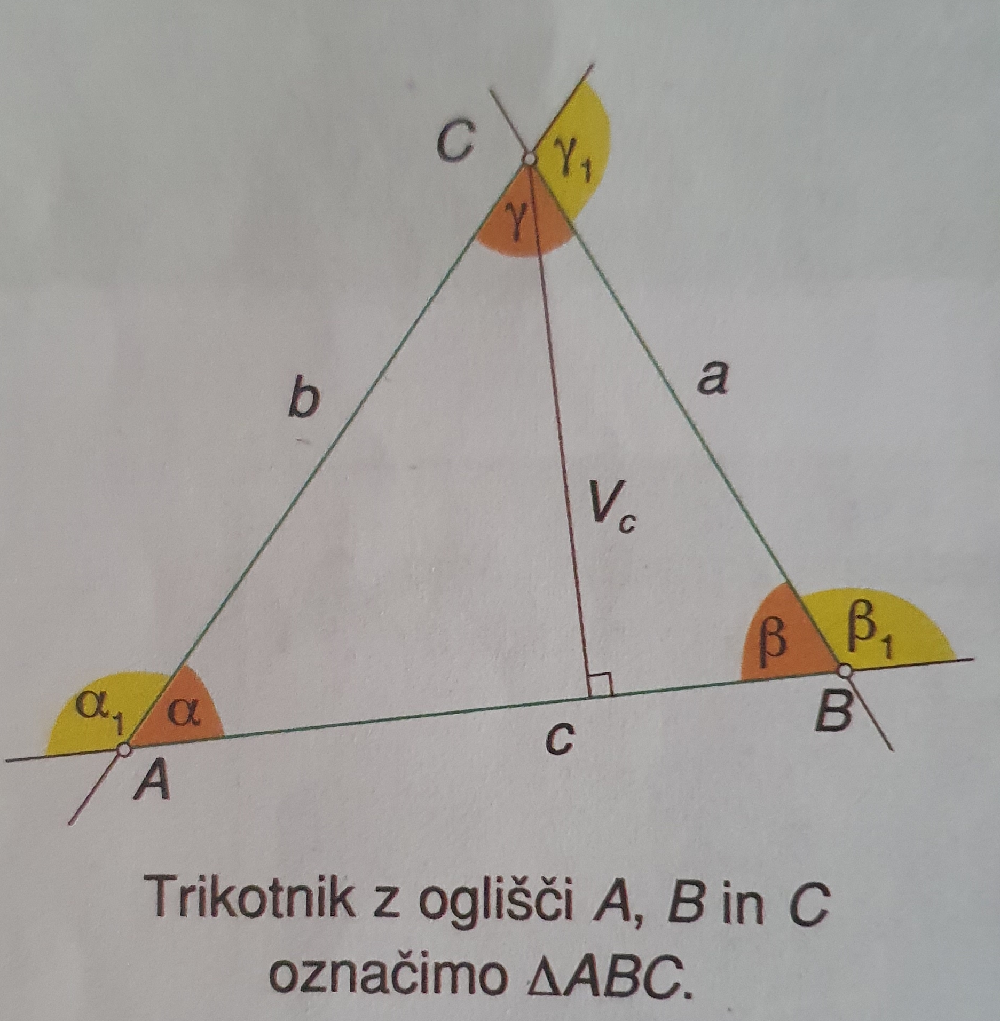
\includegraphics[width=0.4\linewidth]{trikotnik.png}
    \centering
    \caption{Trikotnik $\Delta ABC$.}
\end{figure}

Točke A, B, C imenujemo oglišča.

Daljice, ki te točke povezujejo imenujemo stranice trikotnika.
Stranica a leži nasproti oglišča A, stranica b nasproti oglišča B in stranica c nasproti oglišča C. Premice, na katerih ležijo stranice trikotnika imenujemo nosilke stranic.

Notranji koti trikonika so koti, ko jih tvorita dve stranici trikotnika.
Kot pri oglišču A  je $\alpha$, pri oglišču B je $\beta$ in pri oglišču C je $\gamma$.

Sokoti notranjih kotov so zunanji koti trikotnika in so $\alpha_1$, $\beta_1$ in $\gamma_1$ ($\alpha'$, $\beta'$ in $\gamma'$).

\begin{figure}[h]
    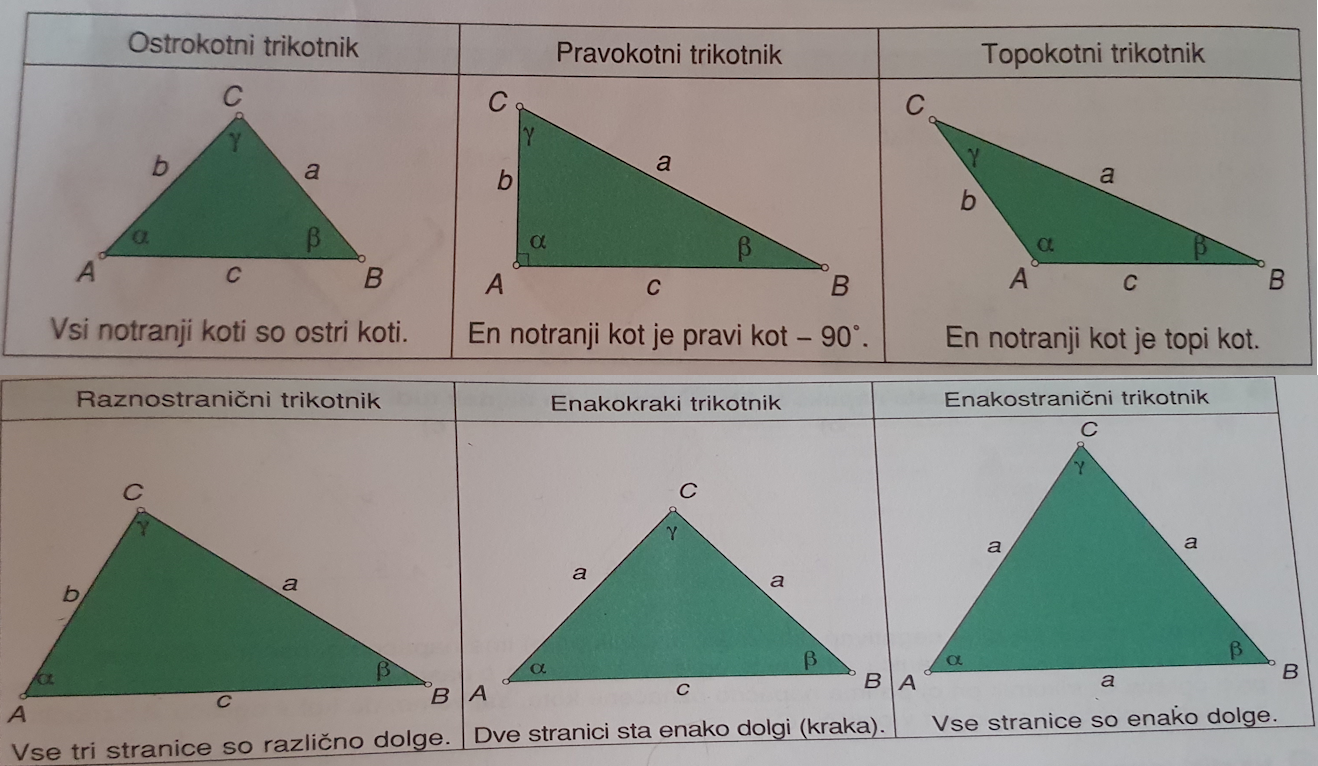
\includegraphics[width=0.7\linewidth]{delitevGledeNaKoteInStranice.png}
    \centering
    \caption{Delitev trikotnikov glede na velikosti notranjih kotov in glede na dolžino stranic.}
\end{figure}

% \begin{figure}[h]
%     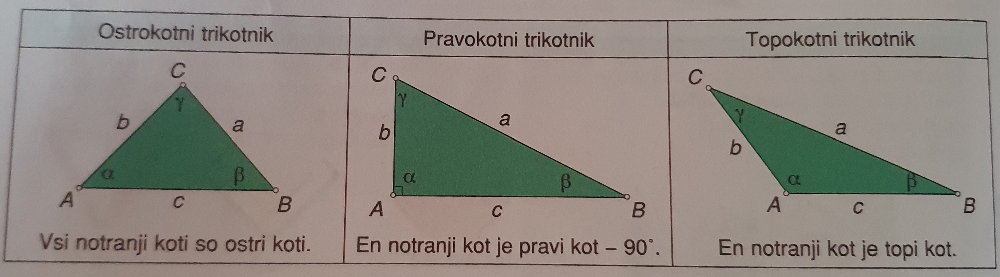
\includegraphics[width=\textwidth]{delitevGledeNaKote.png}
%     \centering
%     \caption{Delitev trikotnikov glede na velikosti notranjih kotov.}
% \end{figure}

% \begin{figure}[h]
%     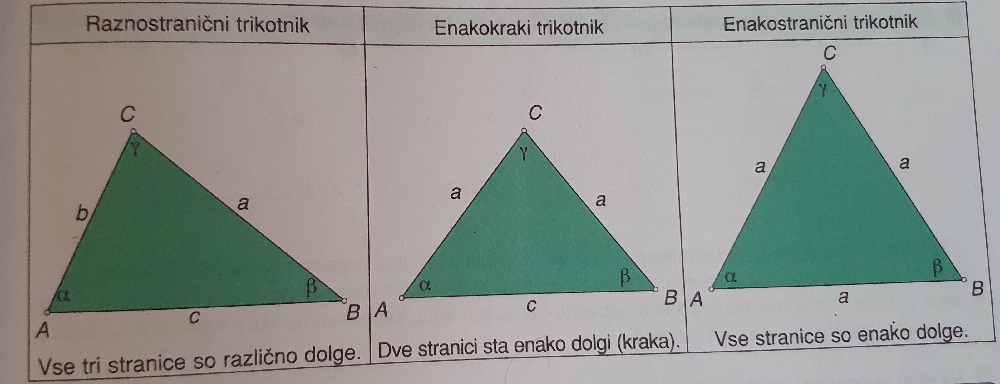
\includegraphics[width=\textwidth]{delitevGledeNaStranice.png}
%     \centering
%     \caption{Delitev trikotnikov glede na dolžino stranic.}
% \end{figure}


\begin{trditev}[Trikotniško pravilo]
    Vsota dolžin dveh stranic v trikotniku mora biti večja od dolžine tretje stranice.
    \[
      a + b > c \quad\quad  a + c > b \quad\quad  b + c > a  
    \]
\end{trditev}


\begin{figure}[h]
    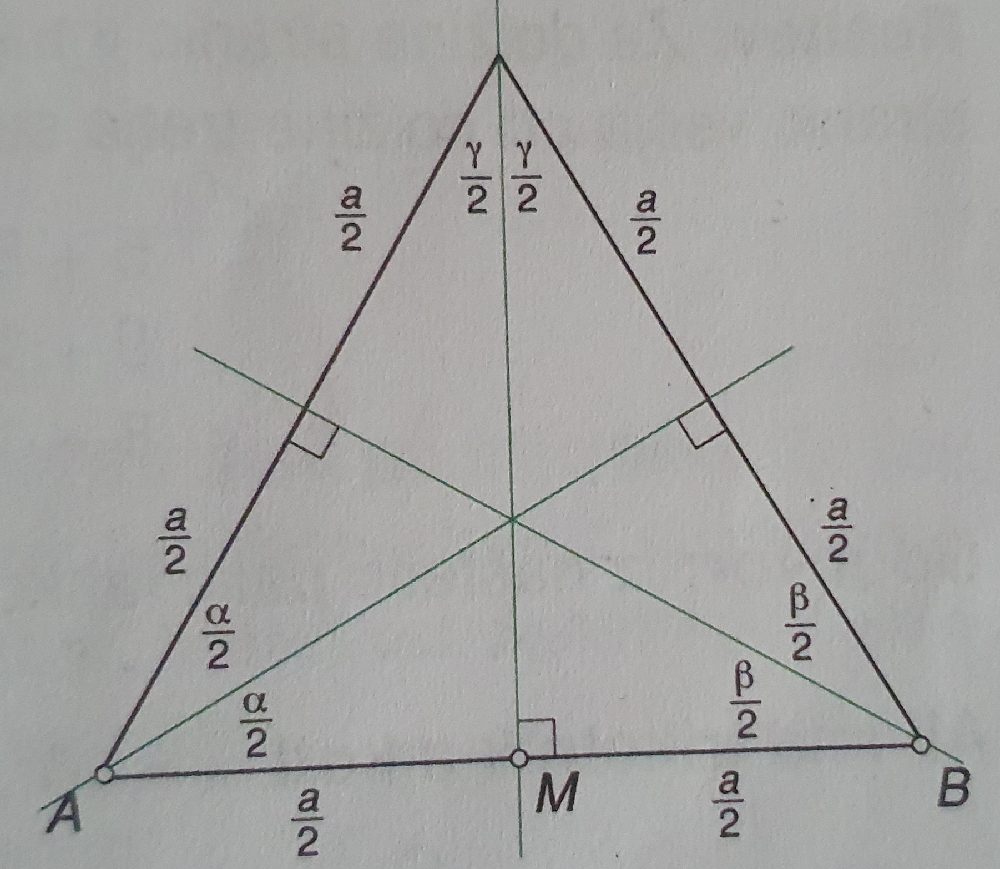
\includegraphics[width=0.5\linewidth]{simetraleEnakostranicni.png}
    \centering
    \caption{Simetrale enakostraničnega trikotnika.}
\end{figure}

Enakostranični trikotnik ima tri simetrale:
\begin{itemize}
    \item vsaka simetrala je pravokotna na stranico in jo razpolavlja,
    \item vsaka simetrala razpolavlja po en noranji kot trikotnika,
    \item vsi notranji koti so skladni: $\alpha = \beta = \gamma = 60^\circ$.
\end{itemize}

\begin{figure}[h]
    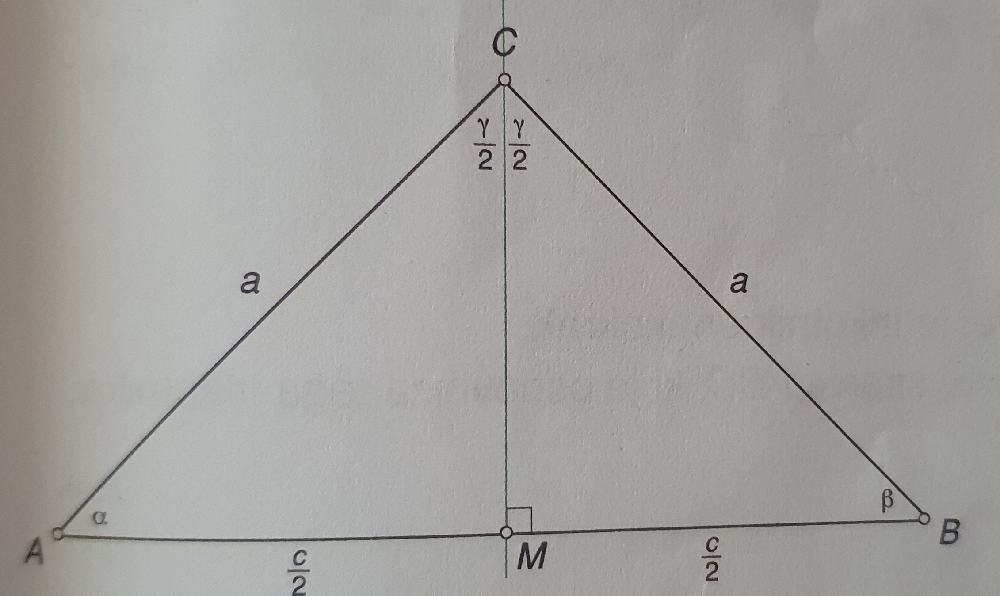
\includegraphics[width=0.5\linewidth]{simetraleEnakokraki.png}
    \centering
    \caption{Simetrale enakokrakega trikotnika.}
\end{figure}

Enakokraki trikotnik ima eno simetralo:
\begin{itemize}
    \item simetrala je pravokotna na osnovnico,
    \item simetrala razpolavlja kot med krakoma,
    \item kota ob osnovnici sta skladna: $\alpha = \beta$.
\end{itemize}

\ \\
Raznostranični trikotnik nima nobene simetrale.

\pagebreak
\subsection{ Koti v trikotniku }

\begin{trditev}
    Vsota notranjih kotov trikotnika je $180^\circ$.
    \[
        \alpha + \beta + \gamma = 180^\circ
    \]
\end{trditev}

\begin{trditev}
    Vsota notranjega in pripadajočega zunanjega kota je $180^\circ$.
    \[
        \alpha + \alpha_1 = 180^\circ \quad\quad
        \beta + \beta_1 = 180^\circ \quad\quad
        \gamma + \gamma_1 = 180^\circ
    \]
\end{trditev}

\begin{trditev}
    Vsota zunanjih kotov trikotnika je $360^\circ$.
    \[
        \alpha_1 + \beta_1 + \gamma_1 = 360^\circ
    \]
\end{trditev}

\begin{trditev}
    Zunanji kot trikotnika je enak vsoti nepriležnih notranjih kotov trikotnika.
\end{trditev}

\begin{figure}[h]
    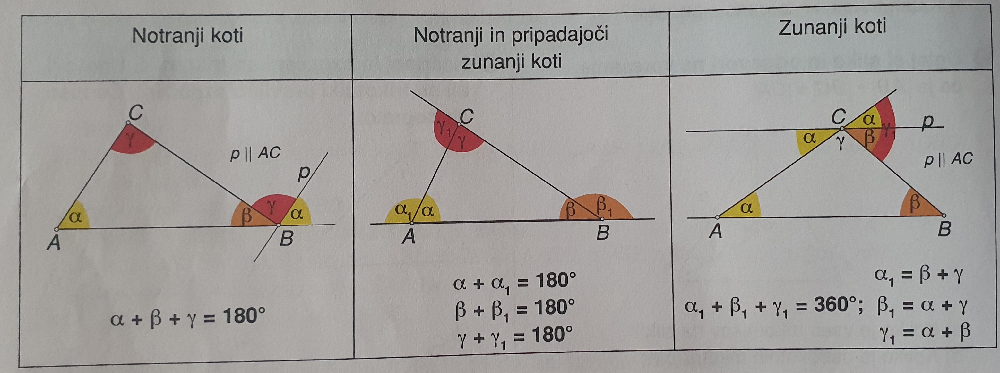
\includegraphics[width=\textwidth]{trditveOKotihTrikotnika.png}
    \centering
    \caption{Grafični prikaz trditev o kotih trikotnika.}
\end{figure}
\begin{figure}[h]
    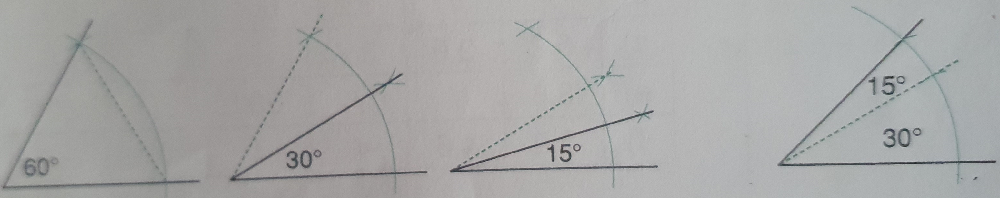
\includegraphics[width=\textwidth]{konstrukcijaKotov.png}
    \centering
    \caption{Konstrukcije kotov $60^\circ$, $30^\circ$, $15^\circ$ in $45^\circ$.}
\end{figure}

\pagebreak
\subsection{ Načrtovanje trikotnikov }

Pri vsakem trikotniku lahko izmerimo šest osnovnih količin: dolžine stranic in velikosti notranjih kotov.

\begin{figure}[h]
    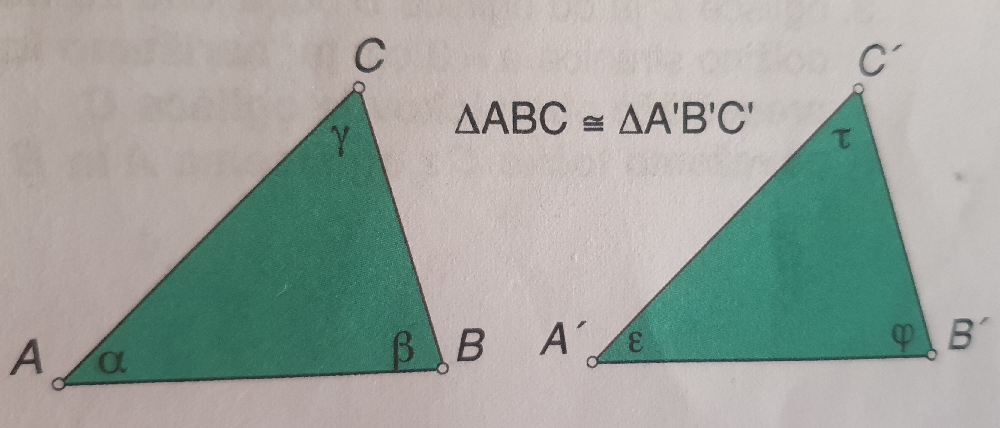
\includegraphics[width=0.8\linewidth]{skladnaTrikotnika.png}
    \centering
    \caption{Skladna trikotnika $\Delta ABC$ in $\Delta A'B'C'$ ($\Delta ABC \cong \Delta A'B'C'$).}
\end{figure}

\begin{definicija}[Skladnost trikotnikov]
    Dva trikotnika sta skladna, če lahko enega premaknemo na drugega, tako da se povsem pokrivata. Ujemata se v vseh treh kotih in vseh treh stranicah.
\end{definicija}

\begin{figure}[h]
    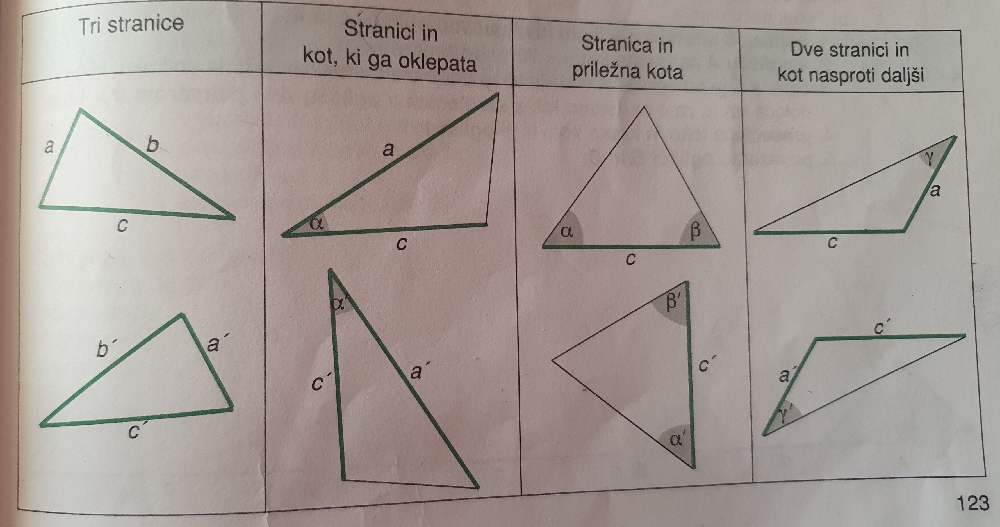
\includegraphics[width=0.8\linewidth]{skladnostniIzrek.png}
    \centering
    \caption{Grafični prikaz skladnostnega izreka.}
\end{figure}

\begin{izrek}[Skladnostni izreki]
    Dva trikotnika sta skladna, če se ujemata v:
    \begin{enumerate}
        \item vseh treh stranicah;
        \item dveh stranicah in kotu, ki ga ti dve stranici oklepata;
        \item eni stranici in dveh priležnih kotih;
        \item dveh stranicah in kotu, ki leži daljši stranici nasproti.
    \end{enumerate}
\end{izrek}


\pagebreak
\subsection{ Višine trikotnikov }

Vsakemu trikotniku lahko določimo tri višine.

\begin{figure}[h]
    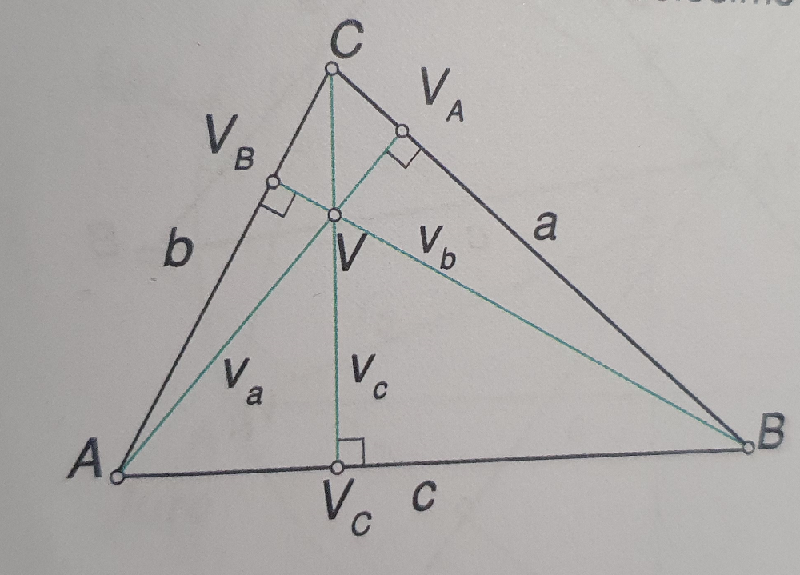
\includegraphics[width=\linewidth]{visineTrikotnika.png}
    \centering
    \caption{Trikotnik z višinami $v_a, v_b, v_c$.}
\end{figure}

\begin{definicija}[Višina trikotnika]
    Višina trikotnika je daljica med ogliščem in nosilko (premico) nasprotne stranice, ki je pravokotna na nosilko (premico) stranice ($v_a, v_b, v_c$). Vse tri višine se sekajo v eni točki, ki jo imenujemo višinska točka (V).
\end{definicija}

\begin{trditev}
    Položaj višinske točke trikotnika je odvisen od velikosti notranjih kotov trikotnika.
    \begin{itemize}
        \item Višinska točka v ostrokotem trikotniku leži v notranjosti trikotnika.
        \item Višinska točka v topokotem trikotniku leži zunaj trikotnika.
        \item Višinska točka v pravokotem trikotniku je oglišče, ki je vrh pravega kota. 
    \end{itemize}
\end{trditev}


\pagebreak
\subsection{ Simetrale stranic in trikotniku očrtana krožnica }

\begin{figure}[h]
    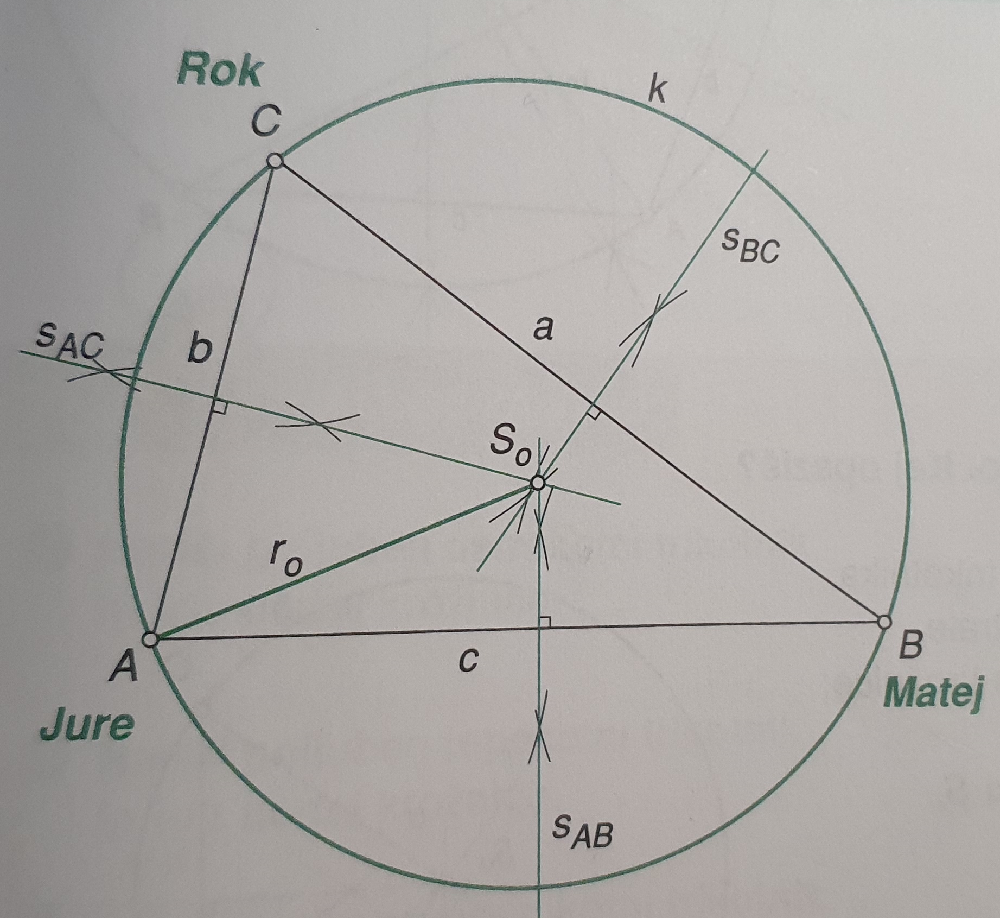
\includegraphics[width=\linewidth]{ocrtanaKroznica.png}
    \centering
    \caption{Očrtana krožnica trikotnika $\Delta ABC$.}
\end{figure}

\begin{definicija}[Simetrala stranice]
    Simetrala stranice so vse točke, ki so enako oddaljene od dveh oglišč trikotnika.
\end{definicija}

Če narišemo vse tri simetrale stranic, dobimo točko, ki je enako oddaljena od vseh treh oglišč trikotnika. Ta točka je središče trikotniku očrtane krožnice. Označimo jo z $S_o$. Razdalja od središča trikotniku očrtane krožnice do kateregakoli oglišča trikotnika je polmer trikotniku očrtane krožnice ($r_o$).


\pagebreak
\subsection{ Simetrale kotov in trikotniku včrtana krožnica }

\begin{figure}[h]
    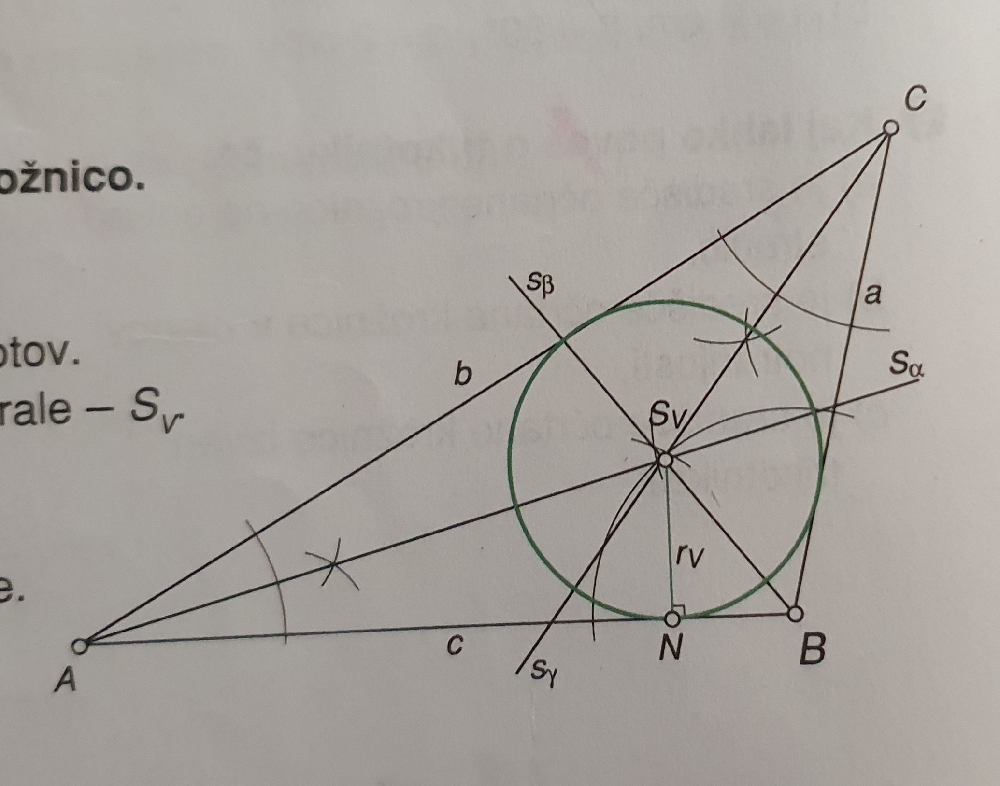
\includegraphics[width=\linewidth]{vcrtanaKroznica.png}
    \centering
    \caption{Včrtana krožnica trikotnika $\Delta ABC$.}
\end{figure}

\begin{definicija}
    Simetrala kota so vse točke, ki so enako oddaljene od dveh stranic trikotnika, ki se v kotu dotikata/stikata. 
\end{definicija}

Če poiščemo simetrale vseh kotov dobimo točko, ki je enako oddaljena od vseh treh stranic trikotnika. Ta točka je središče trikotniku včrtane krožnice. Označimo jo z $S_v$. Razdalja od središča trikotniku včrtane krožnice $S_v$ do poljubne stranice trikotnika je polmer včrtane krožnice ($r_v$).


\pagebreak
\subsection{ Težiščnice in težišče }

\begin{figure}[h]
    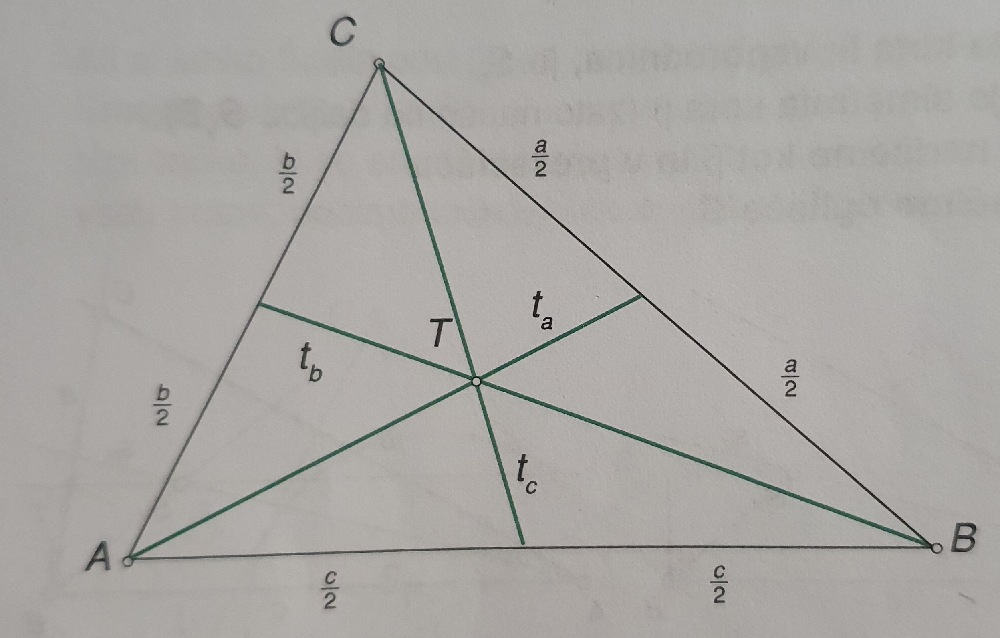
\includegraphics[width=\linewidth]{teziscniceTrikotnika.png}
    \centering
    \caption{ Težiščnice $t_a$, $t_b$ in $t_c$ trikotnika $\Delta ABC$.}
\end{figure}

\begin{definicija}
    Težiščnica trikotnika je daljica, ki povezuje oglišče trikotnika z razpoloviščem nasprotne stranice. Težiščnice trikotnika označimo s $t_a$, $t_b$ in $t_c$. Težišče $T$ trikotnika $\Delta ABC$ je točka, v kateri se sekajo vse tri težiščnice trikotnika.
\end{definicija}

\pagebreak
\subsection{ Štirikotniki }

\begin{definicija}[Štirikotnik]
    Štirikotnik je množica točk v ravnini, ki je omejena s štirimi daljicami.    
\end{definicija}

\begin{figure}[h]
    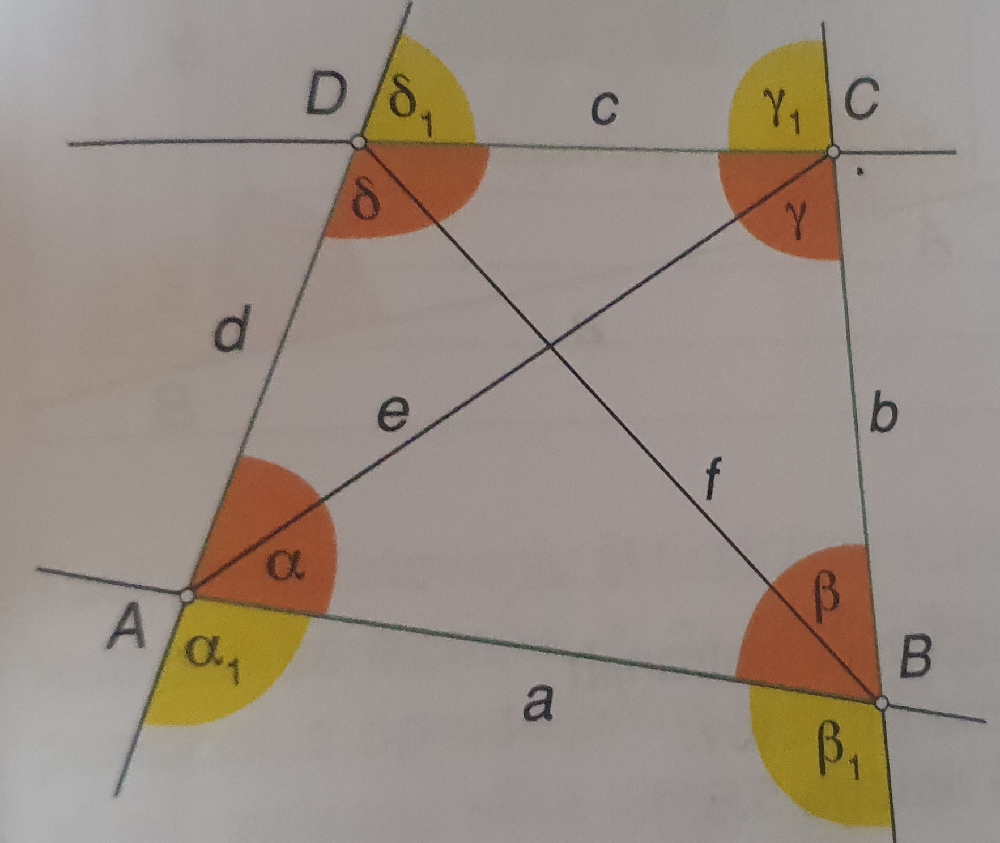
\includegraphics[width=0.7\linewidth]{stirikotnik.png}
    \centering
    \caption{Štirikotnik ABCD.}
\end{figure}

Točke A, B, C in D imenujemo oglišča.

Stranice a, b, c in d so razdalje med sosednimi oglišči.

Nosilke stranic so premice, na katerih ležijo stranice.

Notranji koti štirikotnika $\alpha$, $\beta$, $\gamma$ in $\delta$ so koti v notranjosti štirikotnika, ki jih tvorita dve stranici štirikotnika.

Sokoti notranijim kotom $\alpha_1$, $\beta_1$, $\gamma_1$, $\delta_1$ ($\alpha'$, $\beta'$, $\gamma'$, $\delta'$) so zunanji koti štirikotnika.

Nasprotni oglišči povezujeta diagonali štirikotnika e in f. 

\pagebreak

\begin{figure}[h]
    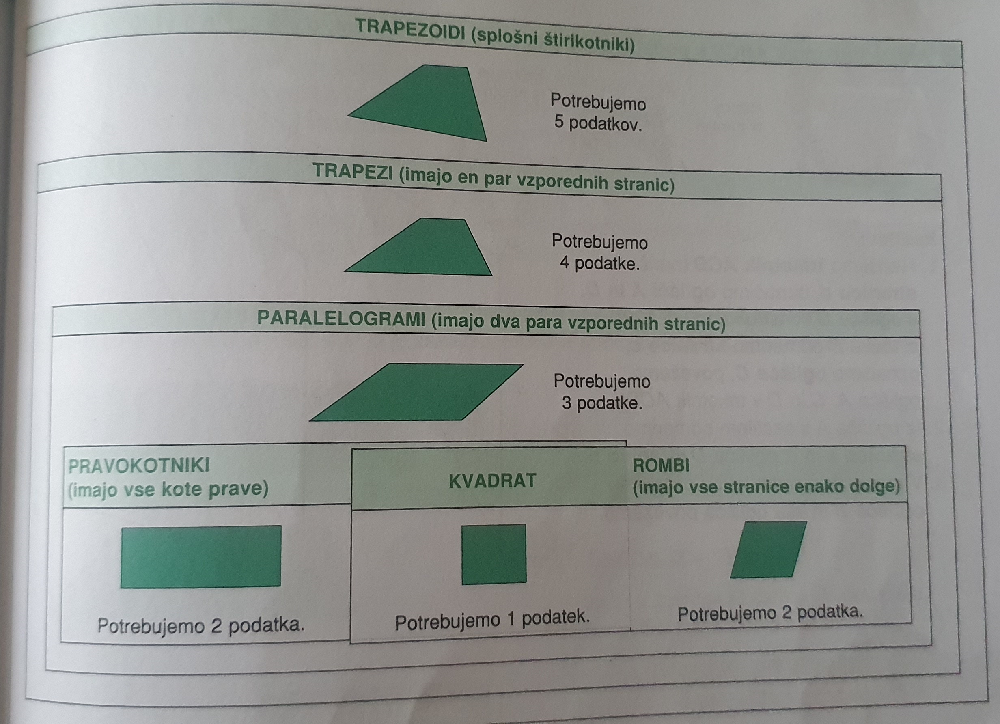
\includegraphics[width=\linewidth]{delitevGledeNaMedsebojnoLegoStranic2.png}
    \centering
    \caption{Delitev štirikotnikov glede na medsebojne lege stranic.}
\end{figure}

\begin{trditev}
    Vsota notranjih kotov štirikotnika je $360^\circ$.
    \[
        \alpha + \beta + \gamma + \delta = 360^\circ
    \]
\end{trditev}

\begin{trditev}
    Vsota notranjega in pripadajočega zunanjega kota je $180^\circ$.
    \[
        \alpha + \alpha_1 = 180^\circ \quad\quad
        \beta + \beta_1 = 180^\circ \quad\quad
        \gamma + \gamma_1 = 180^\circ \quad\quad
        \delta + \delta_1 = 180^\circ
    \]
\end{trditev}

\begin{trditev}
    Vsota zunanjih kotov štirikotnika je $360^\circ$.
    \[
        \alpha_1 + \beta_1 + \gamma_1 + \delta_1 = 360^\circ
    \]
\end{trditev}

\pagebreak
\subsection{ Trapez }

\begin{definicija}[Trapez]
    Trapez je štirikotnik, ki ima en par vzporednih stranic.  
\end{definicija}

\begin{figure}[h]
    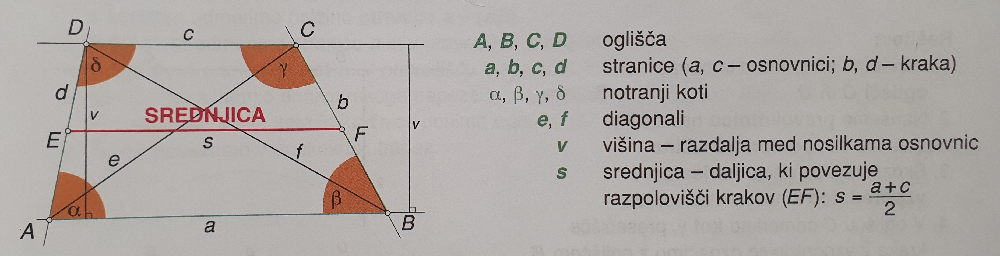
\includegraphics[width=\linewidth]{trapez.png}
    \centering
    \caption{Trapez.}
\end{figure}

\begin{definicija}[Srednica trapeza]
    Srednica trapeza je daljica, ki povezuje razpolovišči obeh krakov: $s = \frac{a + c}{2}$.
\end{definicija}

\begin{figure}[h]
    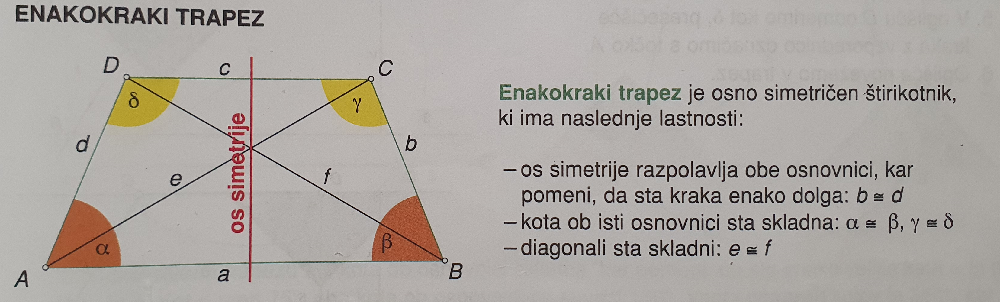
\includegraphics[width=\linewidth]{enakokrakiTrapez.png}
    \centering
    \caption{Enakokraki trapez.}
\end{figure}

\pagebreak
\subsection{ Paralelogram }

\begin{definicija}[Paralelogram]
    Paralelogram je štirikotnik, ki ima dva para vzporednih stranic.  
\end{definicija}

\begin{figure}[h]
    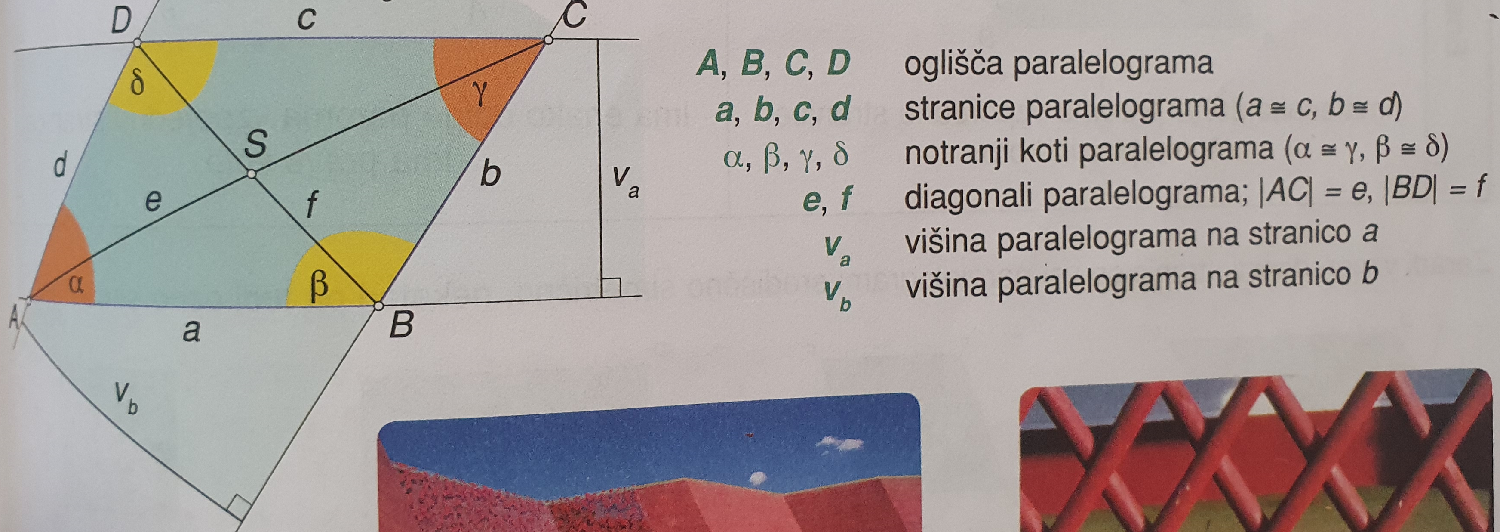
\includegraphics[width=0.9\linewidth]{paralelogram.png}
    \centering
    \caption{Paralelogram.}
\end{figure}


\begin{trditev}
    Paralelogram ima naslednje lastnosti:
    \begin{itemize}
        \item nasprotni stranici sta skladni,
        \item nasprotna kota sta skladna,
        \item kota ob isti stranici sta suplementarna:\\
         $\alpha + \beta = 180^\circ$, $\beta + \gamma = 180^\circ$, $\gamma + \delta = 180^\circ$, $\alpha + \delta = 180^\circ$
        \item diagonali se razpolavljata.
    \end{itemize}
\end{trditev}

\begin{figure}[h]
    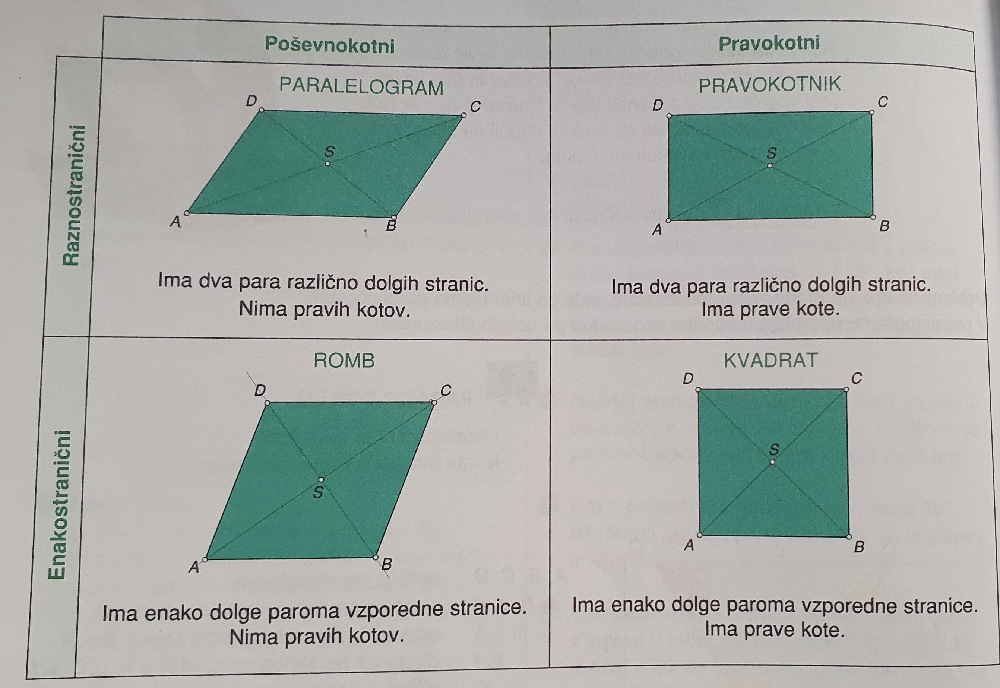
\includegraphics[width=0.9\linewidth]{delitevParalelogramaGledeNaNotranjeKoteInDolzineStranic.png}
    \centering
    \caption{Delitev paralelogramov glede na notranje kote in dolžine stranic.}
\end{figure}

\pagebreak
\subsection{ Deltoid }

\begin{definicija}[Deltoid]
    Deltoid je štirikotnik, ki ima dva para skladnih stranic.  
\end{definicija}

\begin{figure}[h]
    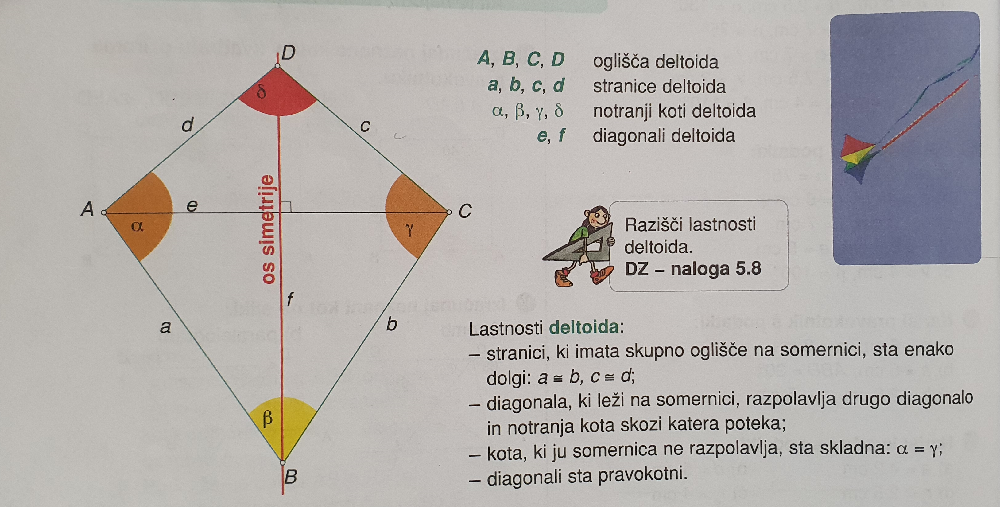
\includegraphics[width=1\linewidth]{deltoid.png}
    \centering
    \caption{Deltoid.}
\end{figure}

\pagebreak
\subsection{ Geometrijski liki in telesa }

\begin{definicija}
    Telo, ki ima za stranske ploskve štirikotnike in dve enaki osnovni ploskvi imenujemo prizma. Telo, ki ima za stranske ploskve trikotnike s skupnim vrhom, imenujemo piramida.
\end{definicija}

\begin{figure}[h]
    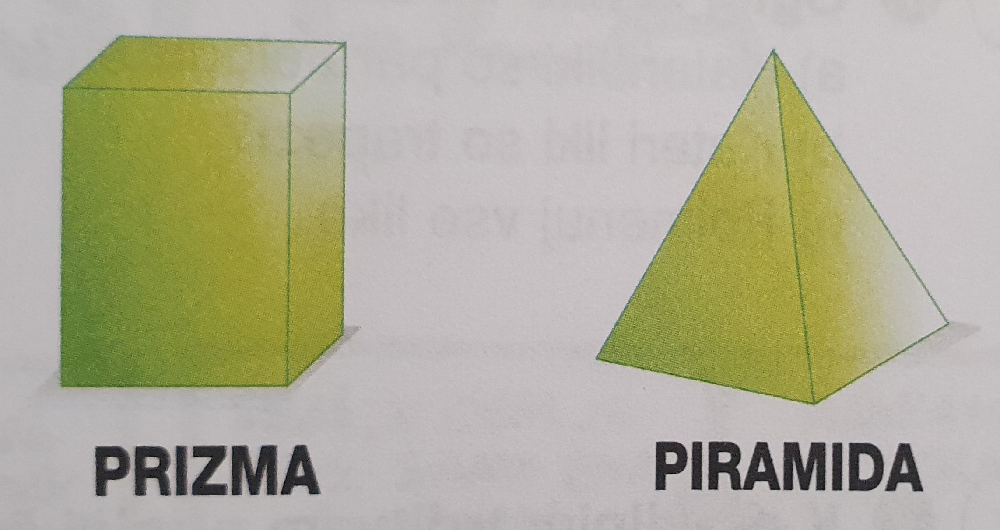
\includegraphics[width=0.7\linewidth]{prizmaInPiramida.png}
    \centering
    \caption{Prizma in piramida.}
\end{figure}

Če ploskve geometrijskega telesa razgrnemo, nastane mreža telesa, iz katere so lepo razvidni geometrijski liki, ki omejujejo telo.


\begin{figure}[h]
    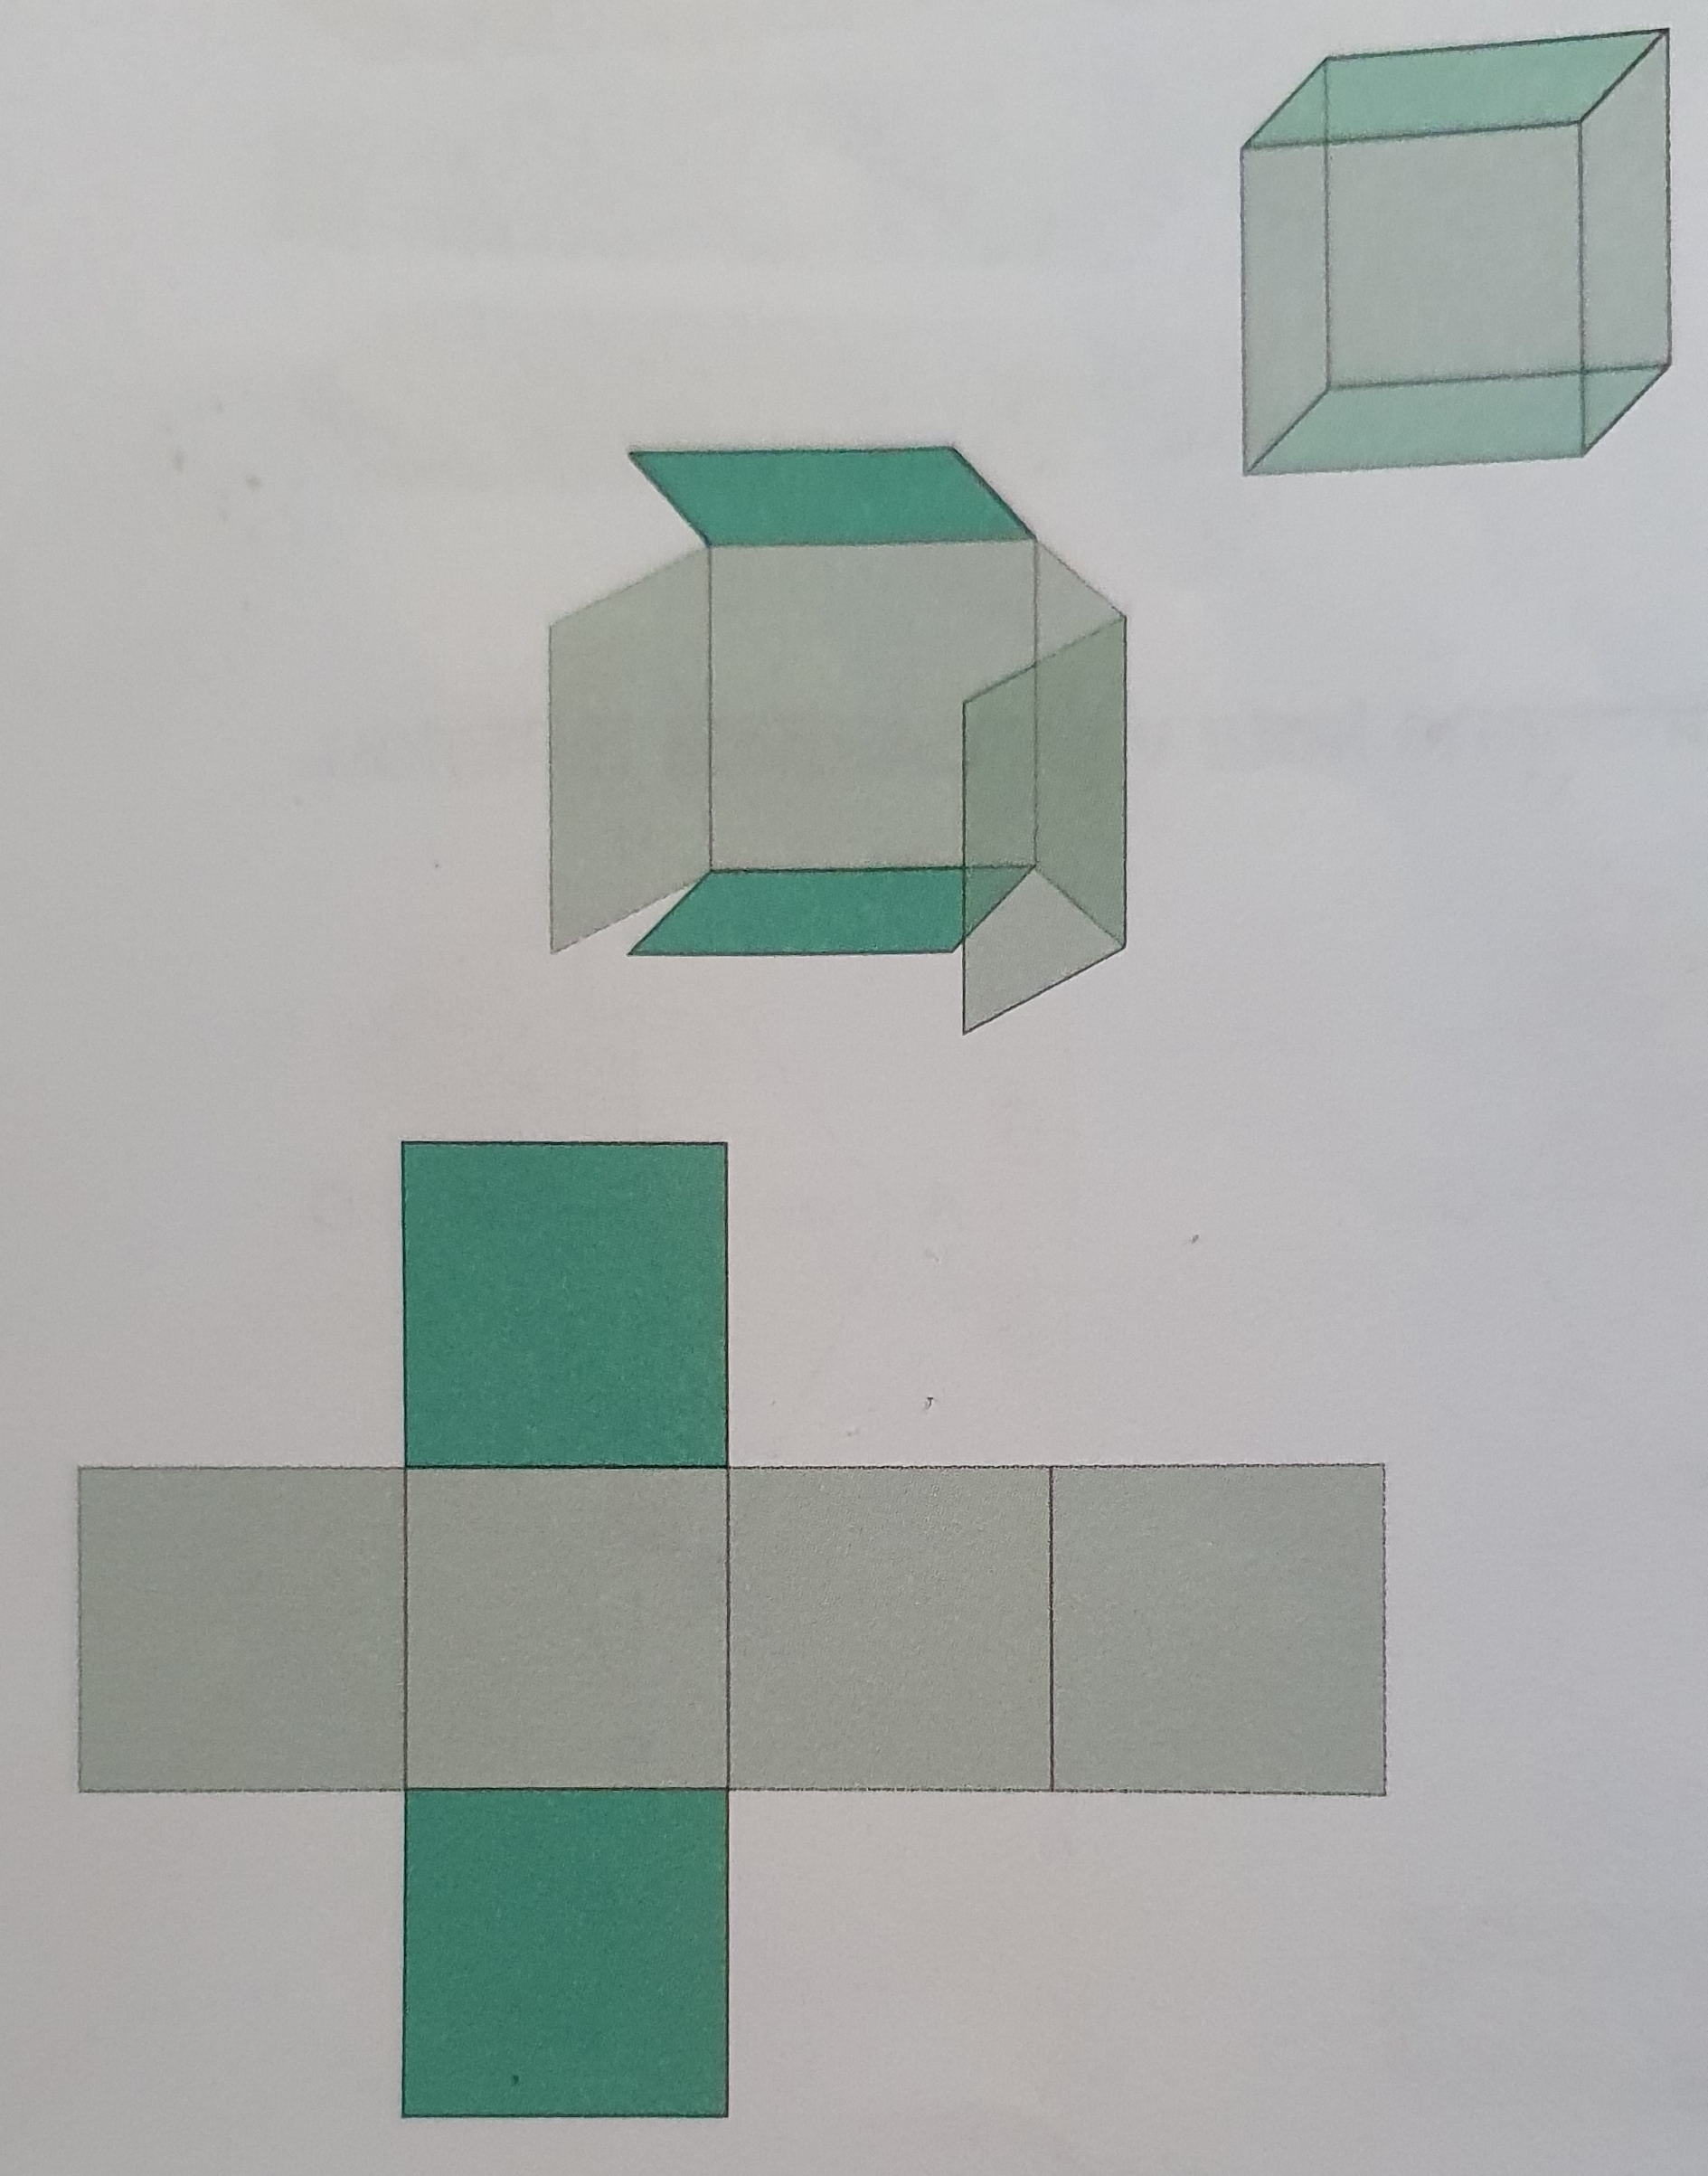
\includegraphics[width=0.5\linewidth]{mrezaKocke.png}
    \centering
    \caption{Mreža kocke.}
\end{figure}





























\end{document}